\chapter{基于纯视觉的堆体体积测量方法研究}
\label{cha:chap4}
\section{引言}
\label{sec:4.1}
利用三维重建的技术流程,可以通过输入二维图片序列的方式获取到场景中的三维稀疏点云或者稠密点云,以视觉的方式来表达场景中的信息。
虽然这些点云可以描绘出空间中的信息,但是还存在以下两个这些问题需要解决:

1)	在三维重建的过程中,由于点云坐标系都是以第一帧的相机为参考坐标系,因此点云坐标系和真实世界坐标系无法对应,对于很多实际应
用场景,都需要获取到该场景的实际水平面,来进行下一步的导航和定位;

2)	由于是单目相机,无法获取特征点的深度信息,因此对于构建出的三维重建点云没有一个绝对尺度的概念。

在解决上述两个问题的基础上,可以对空间中的封闭物体进行高度,面积或者体积的测算,对比传统方法中用激光雷达等设备来测算体积的方
式,现在就可以通过单个摄像头以纯视觉的方式来完成上述过程,并获取到一个精确的结果。本章将以三维重建的点云结果为基础,为了解决
点云的尺度问题,以及求解三维点云的水平面方程,本文将在场景中引入Aruco二维码,因为Aruco二维码本身携带尺度信息,每一种二维码
都有唯一的ID值,并且其还具备较为容易检出的角点坐标。在获取到尺度和水平面方程后,随后结合点云信息可以再进一步计算三维场景的体
积,具体流程如图~\ref{fig:getVolume}所示。

\begin{figure}[H] % use float package if you want it here
    \centering
    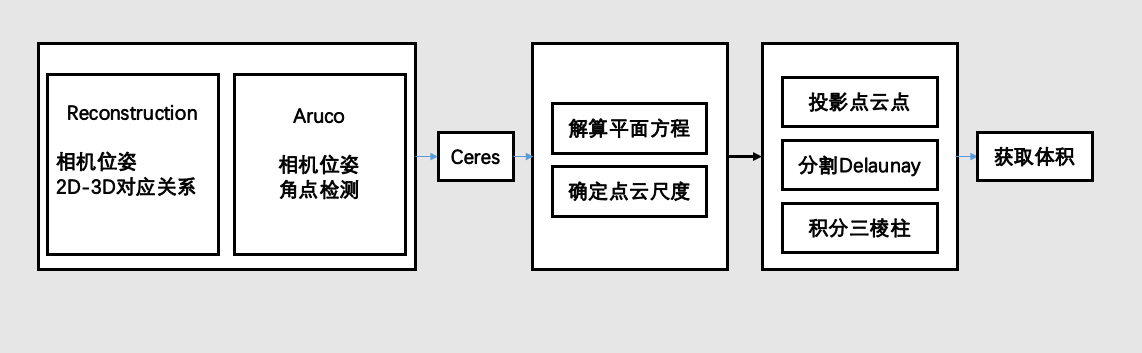
\includegraphics[height=5cm]{getVolume.png}
    \caption{体积测算流程图}
    \label{fig:getVolume}
  \end{figure}

\section{堆体水平面方程解析方法}
\label{sec:4.2}
对于大尺度的场景,都需要得到该场景的水平面所在的平面的方程,由于物体的遮挡,水平面很难直接通过视觉的方法构建出来,从而
导致整个场景非闭合,因此添加水平面后可以使得整个场景封闭;因此,水平面的存在能够更好的计算场景的几何特性,例如场景的高度,
面积,体积等。由于三维重建本身的点云结果都是基于参考坐标系,没有和世界坐标系对齐,本文考虑到可以结合点云中能够获取到世界坐标
系的Aruco二维码作为媒介,进行坐标系的转换,该类型二维码如图~\ref{fig:getVolume_Aruco}所示。
\begin{figure}[H] % use float package if you want it here
  \centering
  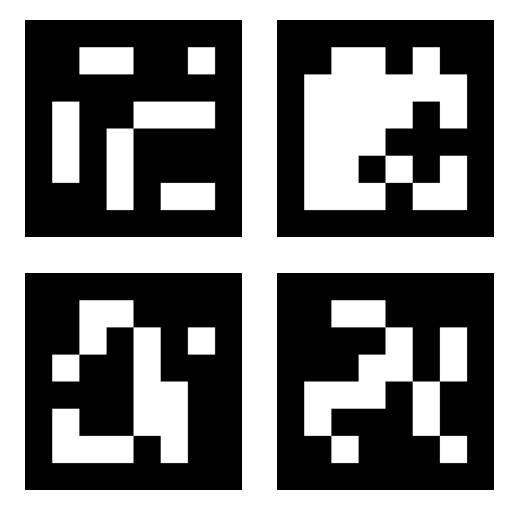
\includegraphics[height=6cm]{getVolume_Aruco.png}
  \caption{多种Aruco示意图}
  \label{fig:getVolume_Aruco}
  \end{figure}
\subsection{2D点坐标检测}
\label{sec:4.2.1}
如图~\ref{fig:getVolume_Aruco_detect}所示,可以利用二维码检测算法检测出场景中二维码的ID值,位置,大小,角点坐标等信息,因为在场景中,
Aruco二维码的布置都会有下侧两个角点直接落在水平面上,因此可以认为所有二维码的下侧角点所构成的平面即是场景的水平面。那么接下
来即可将水平面的求解转化为二维码角点所在平面的求解。在检测的过程中,需要将所有2D图片的索引和角点的位置记录下即可。

\begin{figure}[H] % use float package if you want it here
\centering
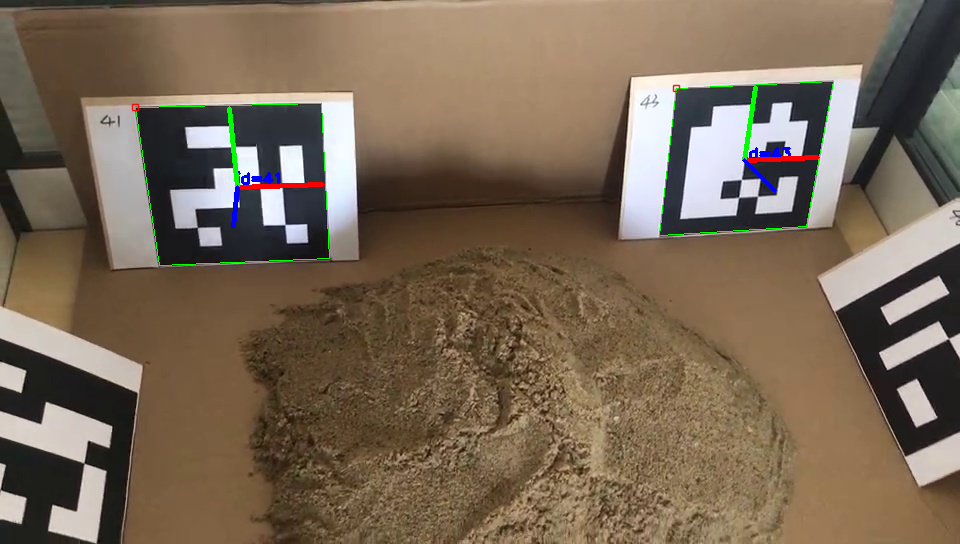
\includegraphics[height=8cm]{getVolume_Aruco_detect_1.png}
\caption{Aruco二维码检测示意图}
\label{fig:getVolume_Aruco_detect}
\end{figure}

\subsection{空间3D点映射方法}
\label{sec:4.2.2}
在上一小结中,可以获得连续视频帧中每一帧的Aruco二维码下侧两个角点的坐标值,同样的,可以直接将这些包含二维码的视频帧序列作为
三维重建的输入以获取场景的点云,考虑到Aruco的角点被作为特征点时极易被检出,因此只需要通过稀疏点云,即可获取角点在二维图像中
的坐标和三维重建点云中的三维坐标之间的对应关系。

在三维重建的过程中,可以获取到每一帧图像中所有特征点所对应的三维重建点云中的三维坐标,无论是稠密点云或者稀疏点云,都可以得到
一个对应关系,但是考虑到遍历的效率问题,则选择稀疏点云中的点击作为遍历对象。在寻找对应关系的实际过程中,会遇到二维坐标无法映
射到三维坐标点的情况,那么则会优先选择距离二维点坐标欧氏距离最近的点作为替代对象。此外,还需要注意的是,若所布置的Aruco二维
码的所有下侧点都位于同一条直线上,那么这样就无法获取准确的水平面方程,因为经过同一直线的平面并不唯一,因此在布置坐标的过程中
需要注意将所有Aruco二维码尽可能对立放置。
\subsection{平面方程解析方法}
根据上述两个步骤,可以将待求的水平面方程问题转化成求解N个三维点所在水平面方程的非线性优化问题。本文选择谷歌开源的Ceres solver
库作为解决该非线性问题的工具,Ceres可以解决边界约束鲁棒非线性最小二乘法优化的问题,表达式如下
\begin{equation}
\begin{array}{l}\underset x{min}\;\;\frac12\sum\rho_i(\parallel f_i(x_{i_1},...,x_{i_k})\parallel^2)
\\s.t.\;\;l_j\leq x_j\leq u_j\\\end{array}
\end{equation}
其中$rho_i(\parallel f_i(x_{i_1},...,x_{i_k})\parallel^2$这一部分为残差块, $f_i(.)$为代价函数,代价函数的求解依赖于一系列
参数$[x_{i_1},...,x_{i_k}]$,所有参数构成参数块,限制边界分别为$l_j$,$u_j$。$rho_i$为损失函数,其作用是减少异常值对优化结果的影响。
在利用Ceres解决非线性问题时,通常分为以下三个步骤:\\
1.	构建代价函数,也就是具体问题所对应的目标式,本小结具体解决N个三维点所在水平面的方程;\\
2.	通过代价函数构建待求解的优化问题;\\
3.	配置求解器参数并求解问题,在这一过程中主要是设定求解方程的方式。\\
上述步骤如代码~\ref{code:chap3:get_plane}所示。
\begin{lstlisting}[
  language=C++,
  numbers=left,                
  numberstyle=\footnotesize,
  frame=single,     
  basicstyle=\small\tt,    
  escapeinside = '',
  caption={获取平面方程参数的~C++~实现},
  label={code:chap3:get_plane}]
  vector<vector<float>> plane_data1;
  vector<float> planex_data1 ,planey_data1, planez_data1;'//待优化量'
  '// 第一部分:构建代价函数模型'
  struct CURVE_FITTING_COST_plane
  {
    CURVE_FITTING_COST_plane (double x,double y,double z)
    :_x( x ), _y ( y ), _z ( z ) {}
    '// 残差的计算'
    template <typename T>
    bool operator() (
      const T* const plane,    
      T* residual ) const 
    {
      residual[0] = plane[0]*T(_x) + plane[1]*T(_y) 
                  + plane[2]*T(_z) + plane[3]; 
      return true;
    }
    const double _x, _y, _z;
  };

  int main ( int argc, char** argv )
  {   
    double plane[4] = {0.1,0.1,0.2,0};
    '// 第二部分:构建最小二乘问题'
    ceres::Problem problem2;
    for ( int i=0; i<planex_data1.size(); i++ ){
      problem2.AddResidualBlock 
      (new ceres::AutoDiffFunction<CURVE_FITTING_COST_plane,1,4> 
      (new CURVE_FITTING_COST_plane 
      (planex_data1[i], planey_data1[i],planez_data1[i])),
      nullptr,
      plane);
    }
    '// 第三部分:配置求解器'
    ceres::Solver::Options options2;    
    options2.linear_solver_type = ceres::DENSE_QR;
    options2.minimizer_progress_to_stdout = true; 
    ceres::Solver::Summary summary2;                 
    ceres::Solve ( options2, &problem2, &summary2 );
    for ( auto a:plane ) {
      outfile_kabc<<a*1/plane[3]<<endl;
      }
    return 0;
  }
\end{lstlisting}
对于任意平面方程,都可以利用以下方程通过确定4个参数的方式来确定唯一解析解。
\begin{equation}Ax+By+Cz+D= 0\label{equ:plane}\end{equation}
在迭代的过程中,同时需要确定每个带估计参数的初始值,最终可以得到方程的四个参数a,b,c,d。

\section{堆体尺度估计方法}
\label{sec:4.3}
由单目视觉重建出来的点云地图都存在没有一个确定尺度的问题,地图中的特征点坐标和相机的位姿都是相对尺度,即最常见的采
取初始化成功后的前两帧作为单位尺度,后续的所有关键帧都以此为参考确定尺度。这样的做法可以获取到地图中所有描述的绝
对尺度,但无法计算出实际尺度,本文提出两种估计尺度大小的方法,这两种方法都主要是通过在场景中引入已知尺度的二维码
来确定所构点云地图的真实尺度,主要针对同一场景,通过计算两种SLAM的相机位姿或者两种SLAM中地图点坐标来确定相对尺度
和绝对尺度之间的比例,从而确定绝对尺度。
\subsection{位姿法解算尺度}
首先,获取绝对尺度的数据,由图~\ref{fig:getVolume_Aruco_detect}所示同时可以得到相机在某一个确定的Aruco下的位姿,因为二维
码自带确定的边长信息,因此可以得到带有绝对尺度的相机位姿($T_x$,$T_y$,$T_z$)。在实际的工程中需要注意,必须选择不同状态的
相机在同一二维码下的位姿,则可以通过多个图像序列获取到多个不同位姿。

其次,再获取同一批图像序列的相对尺度,通过三维重建的结果,就可以得到每一帧相机在参考坐标系下的位姿($T_x$,$T_y$,$T_z$),
该位姿为相对尺度,因为只需要考虑到尺度的大小关系,因为不需要讨论不同坐标系之间的相对转化问题。

以上可以获取到多个针对同一场景的两种SLAM相机位姿估计结果,接下提出通过位姿来估计尺度的方法因为两种SLAM方法估计出
的相机位姿是基于不同的坐标系得到的,本文提出利用相机在不同坐标系下移动的欧式距离之间的比例来确定尺度,简化公式为:
\begin{equation}K\;=\;\frac{\triangle Pose_{rel}}{\triangle Pose_{abs}}  
\label{equ:getVolume_K}\end{equation}
同4.2.1节,利用Ceres库得到最优解K值,计算如代码~\ref{code:chap3:get_k}所示,
\begin{lstlisting}[
  language=C++,
  numbers=left,                
  numberstyle=\footnotesize,
  frame=single,     
  basicstyle=\small\tt,    
  escapeinside = '',
  caption={获取尺度值的~C++~实现},
  label={code:chap3:get_k}]
  vector<vector<float>> colmap, opencv;
  vector<float> colmap_data1 ,opencv_data1;'//待优化量'
  '// 第一部分:构建代价函数模型'
  struct CURVE_FITTING_COST_k
  {
    CURVE_FITTING_COST_k (double x,double y)
    '// 残差的计算'
    template <typename T>
    bool operator() (
      const T* const k,     
      T* residual ) const     
    {
      residual[0] = T ( _y ) - ( k[0]*T ( _x ) ); // y-ax
      return true;
    }
    const double _x, _y;
  };
  int main ( int argc, char** argv )
  {   
    double k[1] = {0};
    '// 第二部分:构建最小二乘问题'
    ceres::Problem problem;
    for ( int i=0; i<colmap_data1.size(); i++ ){
      problem.AddResidualBlock 
      (new ceres::AutoDiffCostFunction<CURVE_FITTING_COST_k, 1, 1>
      (new CURVE_FITTING_COST_k 
      (opencv_data1[i], colmap_data1[i])),
      nullptr,
      k);
    }
    '// 第三部分:配置求解器'
    ceres::Solver::Options options;   
    options.linear_solver_type = ceres::DENSE_QR;  
    options.minimizer_progress_to_stdout = true;  
    ceres::Solver::Summary summary;              
    ceres::Solve ( options, &problem, &summary );  
    for ( auto a:k ) {
      outfile_kabc<<a<<endl;
      }
  return 0;
  }
\end{lstlisting}
只需要杰出唯一参数K即可,在计算的过程中需要随机获取任意两帧之间的位姿,以减小误差。
\subsection{空间坐标点解算尺度}
对于尺度的估计,可以通过场景中已知点之间的距离通过投影获得点云之中点的实际坐标,但是空间中的已知点难以确定,而且也不易保持固定
不变,符合以上规则的点的数量又较少。因此考虑到场景中二维码标记的角点为研究对象,可以通过SLAM求得每一个二维码在图像中的位置以及
四个角点的位置,因为角点极易识别,且任意两个角点之间的实际空间距离都能够简易测量得到。

通过上一章三维重建的流程,可以获取到每一个点在二维图像中和三维空间点之间的对应关系,如图所示~\ref{fig:getVolume_get_sizebyPoint}
表示的是同一个点在二维和三维之间的对应。因为图像中的任意两个二维码角点之间的距离都是已知的,那么也可以得到三维坐标中任意两个角
点之间的绝对尺度,将这一尺度因子应用到整个地图中进行缩放,即可获得一个带有真实尺度的地图。
\begin{figure}[H] % use float package if you want it here
  \centering
  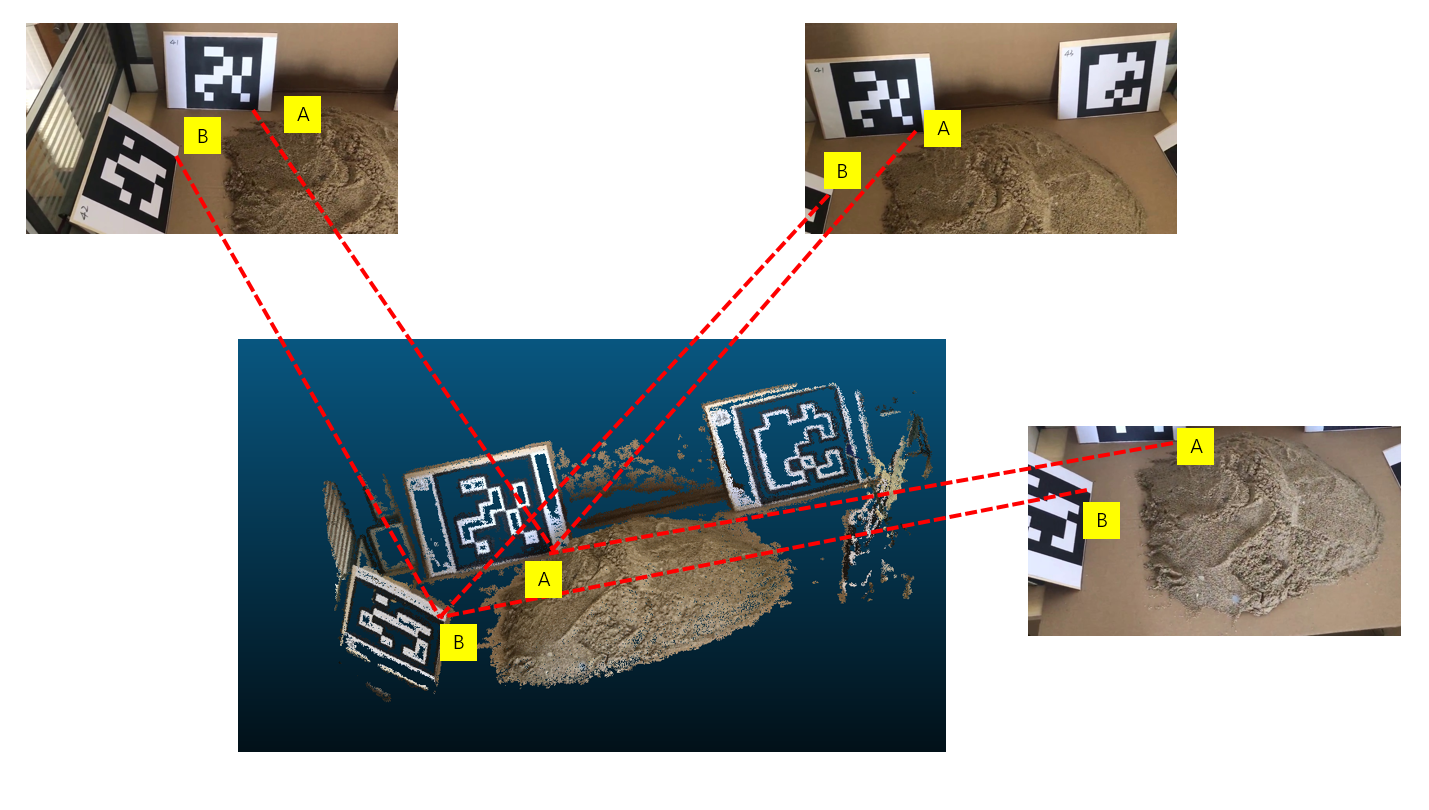
\includegraphics[height=8cm]{getVolume_get_sizebyPoint.png}
  \caption{根据空间点估计尺度流程图}
  \label{fig:getVolume_get_sizebyPoint}
\end{figure}
\section{纯视觉体积测量方法}
\label{sec:4.4}
根据以上两节可以获取到三维重建后点云的水平面和比例尺度,再此基础上计算出物体的实际体积,本文提出一种计算点云实际体积的方法,
具体流程如下:\\
1.	将所有点云结果投影在水平面上,根据场景的实际空间约束和过滤方法提出得到点云中的有效3D点集;\\
2.	通过空间变换,将三维空间点转化为水平面上的点2D点集;\\
3.	对所有点集求Delauncy三角形,计算每个三角形对应的水平高度,得到三棱柱体积;\\
4.	剔除异常三棱柱,将所有有效的三棱柱积分求和得到总体积。
\subsection{有效3D点集获取}
\label{sec:4.4.1}
通过第~\ref{cha:chap3}章的方法,可以对场景获取到三维稀疏点云和稠密点云,在生成点云的过程中会把部分非感兴趣区域的内容和一些
离散的误差噪音点添加至点云结果中。针对这两种情况,本文分别提出以下对应的解决方法:\\
1.	针对非感兴趣区域,本文通过三维空间平面方程对非感兴趣区域直接进行切割剔除;\\
2.	针对随机误差噪音点,本文通过离群点检测算法进行剔除。

对于方案1,在三维重建后的点云中,只需要收集感兴趣区域内的3D点集,如图~\ref{fig:getVolume_interesting}所示,只有红色框图
内区域是感兴趣区域,可以通过上一节求出的水平面方程和二维码的底边点坐标共同约束求出空间切面方程对场景进行切割。
\begin{figure}[H] % use float package if you want it here
  \centering
  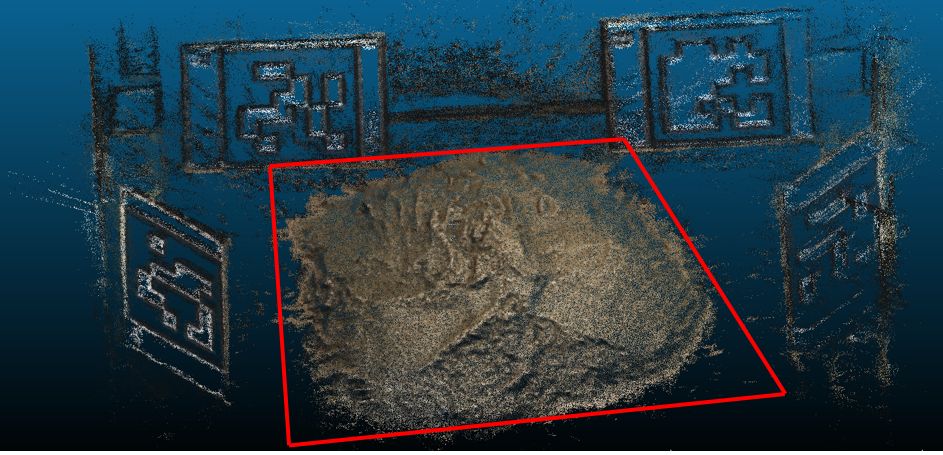
\includegraphics[height=5cm]{getVolume_interesting.png}
  \caption{三维重建感兴趣区域示意图}
  \label{fig:getVolume_interesting}
\end{figure}
对于方案2,本文采用统计滤波器即为对每个点的邻域进行一个统计分析,并修剪掉一些不符合标准的点,具体方法为在输入数据中对点到临
近点的距离分布的计算,对每一个点,计算它到所有临近点的平均距离(假设得到的结果是一个高斯分布,其形状是由均值和标准差决定),
那么平均距离在标准范围之外的点,可以被定义为离群点并从数据中去除。采用统计滤波对点云中的离散点进行滤波对比如
图~\ref{fig:getVolume_3dconstr_filter}所示。
\begin{figure}[H]
  \centering
    \subcaptionbox{对点云统计滤波前}{\label{fig:chap1:getVolume_3dconstr_noise}
    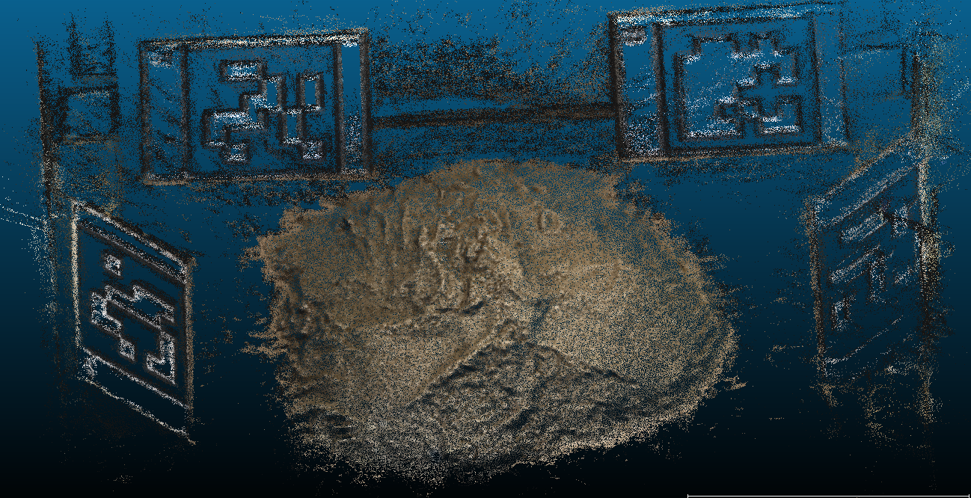
\includegraphics[width=9cm]{getVolume_3dconstr_noise.png}}
  \vskip0.5cm
    \subcaptionbox{对点云统计滤波后}{\label{fig:chap1:getVolume_3dconstr_nonoise}
    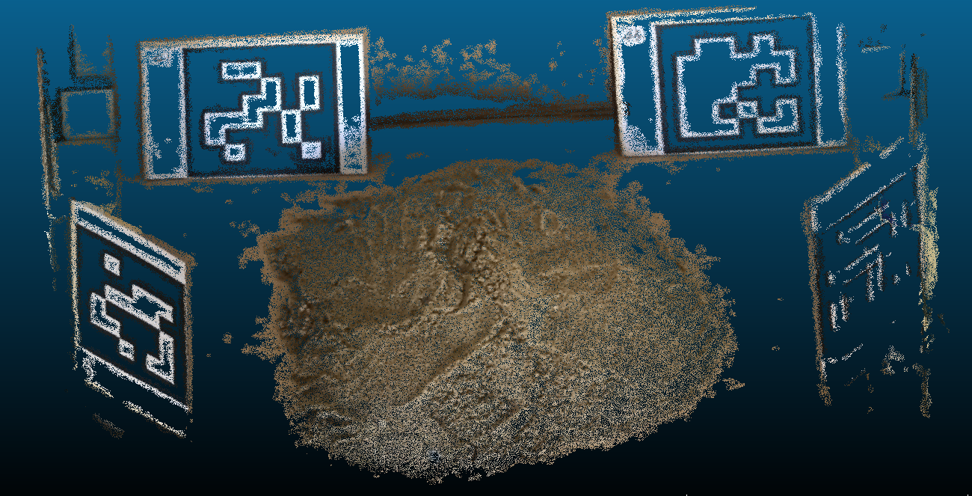
\includegraphics[width=9cm]{getVolume_3dconstr_nonoise.png}}
  \caption{点云统计滤波前后效果对比示意图}\label{fig:getVolume_3dconstr_filter}
\end{figure}

通过上一步骤,可以求出有效的3D点集,接下来需要将所有三维点云投影至二维平面上获取2D点集,简略步骤如下:\\
1.	通过~\ref{sec:4.2}节获取点云水平面和参考坐标系中的xy平面方程的法向量分别为U(A,B,C)和V(0,0,1);\\
2.	将所有的3D点集O($x_o$,$y_o$,$z_o$)根据以下公式投影水平面上,获取新的3D点集P($x_p$,$y_p$,$z_p$);
\begin{equation}
  \begin{split}
  x_p=\frac{(B^2+C^2)x_o-A(By_o+Cz_o+D)}{A^2+B^2+C^2}\\
  y_p=\frac{(A^2+C^2)y_o-B(Ax_o+Cz_o+D)}{A^2+B^2+C^2}\\
  z_p=\frac{(A^2+B^2)z_o-C(Ax_o+By_o+D)}{A^2+B^2+C^2}
  \label{equ:pxyz}
  \end{split}
\end{equation}
同时也可以根据公式计算出每一个三维空间点到水平面的方程的距离
\begin{equation}
d\;=\frac{\left|Ax_0+By_0+Cz_0+D\right|}{\sqrt{A^2+B^2+C^2}}
\end{equation}
3.	计算旋转角度:
\begin{equation}
\theta=arc\cos(\frac{P\cdot Q}{\left|P\right|\left|Q\right|})
\end{equation}
4.	计算旋转轴:在计算旋转角时可知,旋转角所在的平面为有P和Q所构成的平面,那么旋转轴必垂直该平面。
假定旋转前向量为a($a_1$, $a_2$, $a_3$), 旋转后向量为b($b_1$, $b_2$, $b_3$)。由叉乘定义得旋转轴c($c_1$, $c_2$, $c_3$)为
\begin{equation}
\begin{pmatrix}c_1\\c_2\\c_3\end{pmatrix}=\begin{pmatrix}a_2b_3-a_3b_2\\a_3b_1-a_1b_3\\a_1b_2-a_2b_1\end{pmatrix}
\end{equation}
5.	根据罗德里格旋转公式将旋转角,旋转轴的表达转化为旋转矩阵R;\\
6.	将3D点集P($x_p$,$y_p$,$z_p$)右乘上述旋转矩阵R可以得到一系列在同一平面上(所有转变后的点z值都相同)的3D点集,提取所有
3D点的x,y值构成2D点集p($x$,$y$)。
\subsection{Delaunay三角网}
\label{sec:4.4.3}
通过~\ref{sec:4.2}小结,可以得到在由在同一平面上的3D点集转化成的2D点集和每一个2D点集对应的距离值d。在本节中将对2D点集进行
三角剖分,获得Dealunay三角网,Delaunay三角网是一系列相连的但不重叠的三角形的集合, 而且这些三角形的外接圆不包含这个面域的其
他任何点,如图~\ref{fig:getVolume_Delaunay}所示。
\begin{figure}[H] % use float package if you want it here
  \centering
  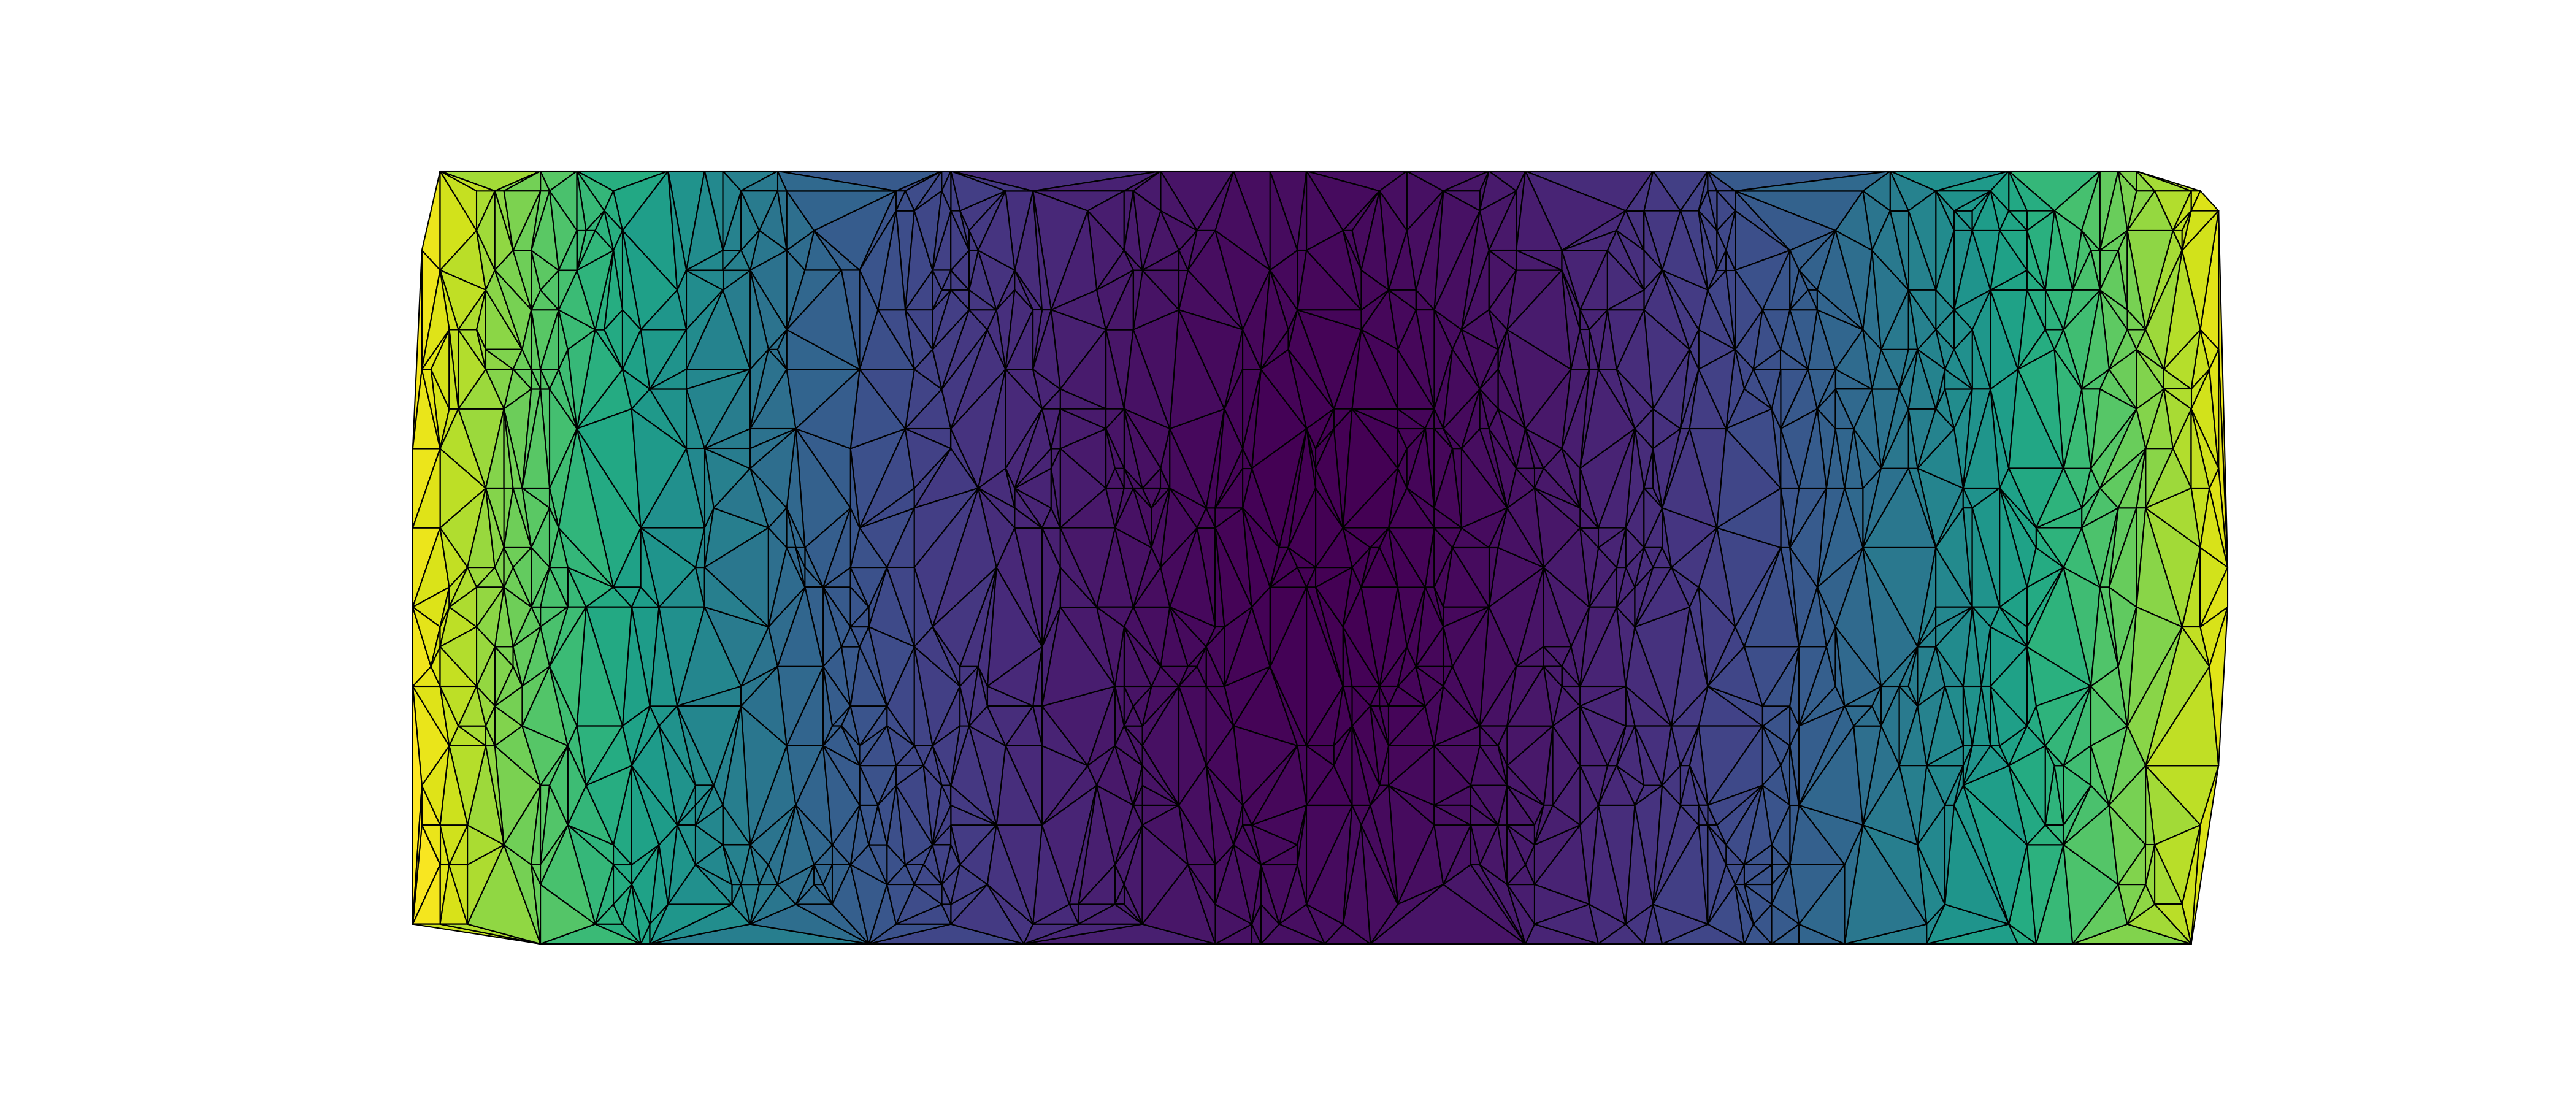
\includegraphics[height=6cm]{getVolume_Delaunay.png}
  \caption{Delaunay三角网示意图}
  \label{fig:getVolume_Delaunay}
\end{figure}
获取Delaunay三角网格的一般步骤为:\\
1.	构造一个超级三角形,包含所有散点,放入三角形链表;\\
2.	将点集中的散点依次插入,在三角形链表中找出其外接圆包含插入点的三角形(称为该点的影响三角形),删除影响三角形的公共边,
将插入点同影响三角形的全部顶点连接起来,从而完成一个点在Delaunay三角形链表中的插入;\\
3.	根据优化准则对局部新形成的三角形进行优化。将形成的三角形放入Delaunay三角形链表;\\
4.	循环执行上述第2步,直到所有散点插入完毕。\\
由于Delaunay剖分具备具备最接近(以最近的三点形成三角形,且各线段(三角形的边)皆不相交)和区域性(新增、删除、移动某一个顶点
时只会影响临近的三角形)的特性,可以对点集所构成的平面进行拟合。通过以上流程可以获得三角形的集合以及三角形中每个顶点对应的距
离,取三个顶点距离的平均值作为三棱柱的高,每个三角形的面积按照公式~\ref{equ:tri_s}计算,即可获得所有三棱柱的体积。
\begin{equation}
S_\bigtriangleup=\frac12\times\left(x_1y_2-x_1y_3+x_2y_3-x_2y_1+x_3y_1-x_2y_2\right)\label{equ:tri_s}
\end{equation}
\subsection{积分三棱柱}
\label{sec:4.4.4}
通过以上步骤,可以将三维重建后点云体积的求解转化成对多个三棱柱积分的求解,因为所有三棱柱的体积值都分布在某一个区间内(并不完
全服从正太分布),对于部分偏差较大的三棱柱体积值应该通过算法进行剔除。本文采用箱形图的方法来处理这一问题,箱形图不受异常值的
影响,能够准确稳定地描绘出数据的离散分布情况,同时也利于数据的清洗。
\begin{figure}[H] % use float package if you want it here
  \centering
  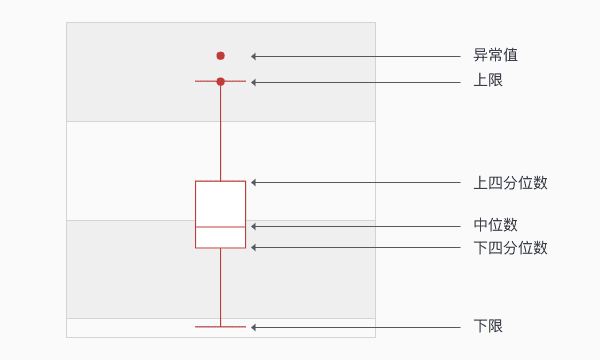
\includegraphics[height=6cm]{getVolume_boxplot.png}
  \caption{Delaunay三角网示意图}
  \label{fig:getVolume_boxplot}
\end{figure}
箱形图如图~\ref{fig:getVolume_boxplot}所示,主要需要求解出数据中的5个特征数据值,包
括下四分位数Q1,上四分位数Q3,四分位距IQR=Q3-Q1,以及上限Q3+1.5IQR和下限Q1-1.5IQR,对于上下限之外的内容需要剔除,最终结
合\label{sec:4.3}所估算出的尺度,以及所有有效三棱柱的体积按照公式~\ref{equ:get_volume}即可估计出物体中感兴趣区域的实际
体积值。
\begin{equation}
  V\;=K^3\;\ast\sum_i\frac13\ast S_\bigtriangleup\times\sum_{j=1}^3d_j\label{equ:get_volume}
\end{equation}
\section{本章小结}
本章的主要目的是通过纯视觉的方式对点云体积进行测量,以获取到堆体的实际体积。

本章提出了通过纯视觉方法进行堆体体积测量的一般步骤,通过位姿比例或空间三维点坐标比例估计出堆体点云和堆体实际空间点之间的尺度关系;通过2D角点获取对应3D映射点,通过非线性优化求解水平面方程参数的最优值;最后再结合水平面投影求解Delaunay三角形,积分三棱柱以估计出堆体点云的体积。

本章所提出方法完全基于视觉方案,整体流程可自动化完成,且可以在相似场景中复用。





